\chapter{Introduzione}
\label{chap:intro}

Questa tesi rappresenta la terza ed ultima parte dello stage++\footnote{Lo stage++ è un progetto unico, formato dall'unione di tre esami: project work, stage e tesi.},
realizzato in collaborazione con e-xtrategy e con il collega e amico Marco D'Argenio.
In questo stage ci è stato chiesto di realizzare un'applicazione per la domotica pensata per l'ufficio che prevedesse l'uso dei beacon, ovvero dei piccoli trasmettitori bluetooth che permetto la geolocalizzazione interna negli edifici. Proprio per questo motivo, il nome che abbiamo deciso di dare al nostro prodotto è: "Proximity System".
Gli obiettivi che dovevamo raggiungere con questo progetto erano numerosi, per questo motivo, io e Marco, ci siamo divisi il carico in maniera bilanciata e logica.
Marco ha trattato gli argomenti relativi al frontend dell'applicazione e ha studiato il BMC\footnote{Business Model Canvas} del progetto per vedere la fattibilità del  progetto da un punto di vista economico, questi argomenti non verranno trattati qui, ma nella tesi di Marco:"Analisi e sviluppo di un sistema software per la domotica d'ufficio: il frontend di Proximity System".
Io, invece, ho trattato tutti gli argomenti inerenti al backend e ai beacon. 
In sintesi, il progetto prevede tre parti: 
\begin{enumerate}
\item Il backend in esecuzione su Raspberry PI
\item Una web app per l'amministrazione del sistema
\item Un'app mobile per gestire i dispositivi
\end{enumerate}
Tutte tre le componenti hanno una cosa in comune, sono tutte scritte in Javascript.
In questa tesi vedremo anche come utilizzare lo stack MEAN\index{MEAN} per lo sviluppo di applicazioni web rispetto al tradizionale stack LAMP e come le WebSocket possano aumentare drasticamente le performance di un'applicazione real-time.

Il codice completo del progetto è disponibile sui due repository\\ www.github.com/e-xtrategy/unicam-beacon-server e\\ www.github.com/e-xtrategy/unicam-ionic-beacon-app. 
Il primo contiene sia il backend con le API REST che la web app in Angular.
Il secondo contiene l'App Ionic compatibile con Android, iOS e, parzialmente (almeno per ora), Ubuntu Touch. 

\section{Analisi e progettazione}
La fase di analisi e di progettazione non si è sviluppata in maniera tradizionale, in quanto e-xtrategy basa lo sviluppo di software sulle metodologie agili, più adatte ad ambienti dinamici come lo è il web.
Fra le pratiche promosse dai metodi agili\index{Agili} ci sono la formazione di team di sviluppo piccoli, cross-funzionali e auto-organizzati, 
lo sviluppo iterativo e incrementale, 
la pianificazione adattiva, 
e il coinvolgimento diretto e continuo del cliente nel processo di sviluppo.

Questa impostazione crea l’esigenza di una piattaforma in grado di tenere traccia dello sviluppo
del software e delle user-stories da implementare, capace anche di coordinare gli sviluppatori
dedicati a quel caso.
Trello\index{Trello}\cite{trello} é un gestore di progetti basato sul web, originariamente realizzato da Fog Creek Soft-
ware nel 2011.
Trello utilizza il paradigma Kanban per la gestione dei progetti. Quest’ultimi sono rappresentati
da schede, che contengono liste corrispondenti ad elenchi di attivitá. Le liste sono formate da
card, che rappresentano le singole attivitá. Le card sono tenute a passare da una lista all’altra,
tramite la funzione drag-and-drop; per via del generico flusso di una card, essa dovrebbe passare
dalla lista delle cose da fare a quelle fatte, al momento del passaggio dall’idea alla realizzazione
dell’attivitá in questione.
Nello specifico le card rappresentano le user-stories, funzionalitá utile al raggiungimento di un
obbiettivo di business, una descrizione appositamente non dettagliata che il software deve avere
e che alimenti la discussione tra il cliente/utente e lo sviluppatore.
Piú programmatori possono essere assegnati alle card, ed insieme alle relative schede, possono
essere raggruppati in organizzazioni differenti. Ogni card puó accettare commenti, allegati, voti,
date di scadenza e liste di controllo.
La suddivisione di un progetto in schede/liste, a loro volta suddivise in card formano una
gerarchia di dati su misura che facilita la gestione efficace dei progetti stessi, nonché delle attività dell'intera organizzazione.
\begin{figure}[h]
\centering
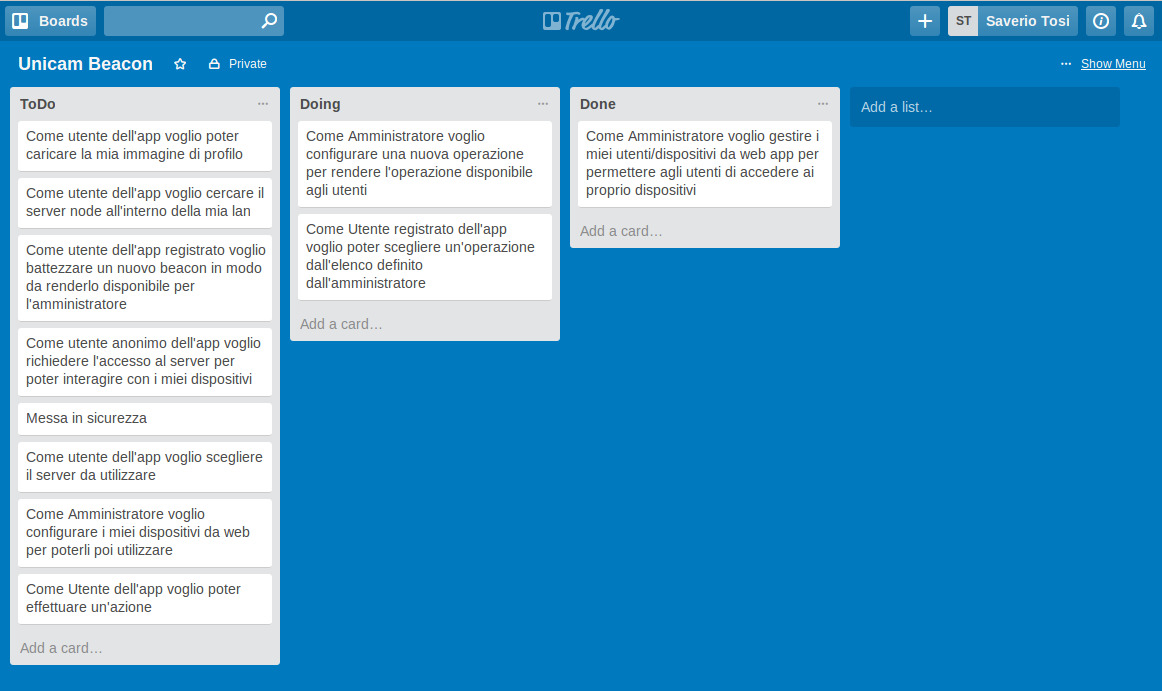
\includegraphics[scale=0.35]{Immagini/trello.png} 
\caption{Il nostro Trello, nella fase iniziale del progetto}
\end{figure}

\subsection{Analisi dei requisiti}
Si vuole realizzare un sistema domotico per l'ufficio, che oltre ad essere comandato con un'app, utilizzi i beacon per eseguire dei comandi automatizzati.

Il backend dove essere caricato su un RaspberryPI 2 e deve fornire i servizi REST sia per la webapp che per l'app mobile. 
Il backend oltre a fornire le API REST\index{REST} dove essere in grado di comunicare con il mondo esterno, sia con input che con degli output.
Per il prototipo, gli input saranno simulati con l'utilizzo di bottoni, nel prodotto finito essi saranno sostituiti con degli interruttori e dei sensori.
Gli output devono pilotare dei relè monostabili che permetteranno di comandare l'accensione/spegnimenti di luci, l'apertura di porte e di cancelli.

Il pannello di amministrazione è rappresentato dalla webapp a cui potrà accedere soltanto l'admin. Essa permette all'admin di gestire gli utenti dell'app dandogli e togliendogli privilegi, tramite la webapp può creare nuovi dispositivi da associare ai vari GPIO del RaspberryPI, infine deve dargli la possibilità di configurare il modo in cui gli utenti possono interagire con i dispositivi: in maniera manuale, automatica(tramite beacon) o se per poter contrallare il dispositivo è necessario trovarsi nelle vicinanze di esso. 

L'ultima componente è l'app mobile. 
Chi scaricherà l'app dovrà per prima cosa impostare l'indirizzo del server, se non si conosce l'indirizzo deve essere possibile fara una scansione della rete locale per trovare i backend attivi nella propria LAN. 
Una volta che si è connessi al server si può proseguire con il login/registrazione. La registrazione non abilita l'utente all'utilizzo di Proximity System, l'utente non potrà far nulla finche l'admin non gli dà i permessi per utilizzare l'app. 
Con l'app un utente ha due funzionalità: la prima è poter cercare nuovi beacon da segnalare all'amministratore; la seconda è interagire con i propri dispositivi.

{\Huge NOTA *** AGGIUNGERE DIAGRAMMA UML PER UTILIZZO APP ***}

\section{Miglioramento dell'esperienza utente}
Dopo una prima stesura del codice e la realizzazione di un primo prototipo,
abbiamo deciso migliorare l'esperienza utente dando la possibilità al server di inviare notifiche push ai due client.
Per fare ciò, abbiamo utilizzato le WebSocket, una delle funzionalità più interessanti introdotta con l'HTML5.

Nel Capitolo \ref{chap:websocket} illustreremo come sia possibile migliorare le  prestazione di una generica WebApp che fornisce dei dati in tempo reale, per poi dimostrare come sia semplice utilizzare tale specifica, sopratutto se si utilizzano delle libreria ad hoc come Socket.io. 